% O treinamento de uma rede neural de convolução~\footnote{\url{http://caffe.berkeleyvision.org/}} foi realizado, utilizando as classes ``praia'' e ``montanha'', balanceadas, da base COREL-1000. A classificação sobre este treinamento obteve $\approx 80\%$ de acurácia, enquanto que utilizando os extratores padrões foi possível atingir apenas $\approx 69\%$. Isso reforça a proposta de analisar quais são as características latentes que esse tipo de rede neural consegue extrair. Para essa análise vão ser utilizadas bases discriminadas quanto às propriedades de textura, cor e forma.

% Não foi testado uma porcentagem fixa para verificar se existe algum ganho em utilizar
% uma ponderação específica.

% é possível melhorar muito os resultados se fazer tunning

Os resultados encontrados apontam para uma alternativa -- ou adição -- a seleção de características, ao usar os métodos de quantização de imagens. Dado o número de cores limitado na imagem original, a quantidade de possíveis características a serem extraídas é reduzido, especialmente as de cor. A extração de características de textura também é facilitada, considerando que normalmente computa utilizando uma memória proporcional o número de intensidades.

Ficou constatado que um vetor original de $D$ dimensões pode ser reduzido a $d \approx D/4$ modifcando apenas o parâmetro de quantização e produzindo bons resultados. Outra possibilidade é utilizar esses métodos como um primeiro passo de redução e então utilizar o LPP para obter apenas 100 características que melhor representam os dados, atingindo acurácias maiores ou similares.

É importante ressaltar que realizar a quantização de imagens não requer treinamento e já faz parte de uma tarefa do pipeline de reconhecimento. Por esta razão, seu uso não aumenta o custo computacional do sistema, e ainda simplifica os passos subsequentes. Isso reduz a dimensão do vetor de características para os vetores de cor e o tempo de computação para os descritores de textura. Outra observação importante é que a quantização é usada especialmente para dados visuais, então não é um método geral de redução de dimensionalidade.

Com os experimentos realizados foi possível notar que a geração de imagens artificiais pode gerar novas informações para a classificação das imagens. Assim a geração de elementos no espaço visual provou contribuir com o balanceamento entre classes (em se tratando de problemas de classes desbalanceadas), melhorando a acurácia de algoritmos de classificação, quando comparada à geração de exemplos artificiais no espaço de atributos (i.e.\ SMOTE). Para validar a ideia da geração artificial de imagens, as características das novas imagens -- extraídas com o método BIC  -- e os exemplos resultantes da interpolação de vetores originais foram projetados no plano das imagens originais antes do desbalanceamento. Dessa forma foi possível visualizar que a geração de imagens artificiais proposta foi capaz de ocupar uma região do espaço mais abrangente do que o SMOTE. Este último, comprovadamente, possui o ponto negativo de não extrapolar os limites da classe minoritária. Ainda, está suscetível à criação de novos exemplos em regiões da classe majoritária, o que também prejudica a classificação.

% A visualização do espaço de características utilizando a técnica de análise de componentes principais (PCA) se mostrou crucial para confirmar visualmente que a melhora da acurácia da classificação se deve à melhor definição da classe minoritária.

\section{Publicações}

Foi publicado um artigo na revista \textit{Neurocomputing} (Figura \ref{fig:artigo}), referente aos resultados de quantização desta pesquisa. O artigo referente à geração de imagens artificiais para o rebalanceamento de classes está em preparo.

\begin{figure}[hbpt]
 \begin{center}
   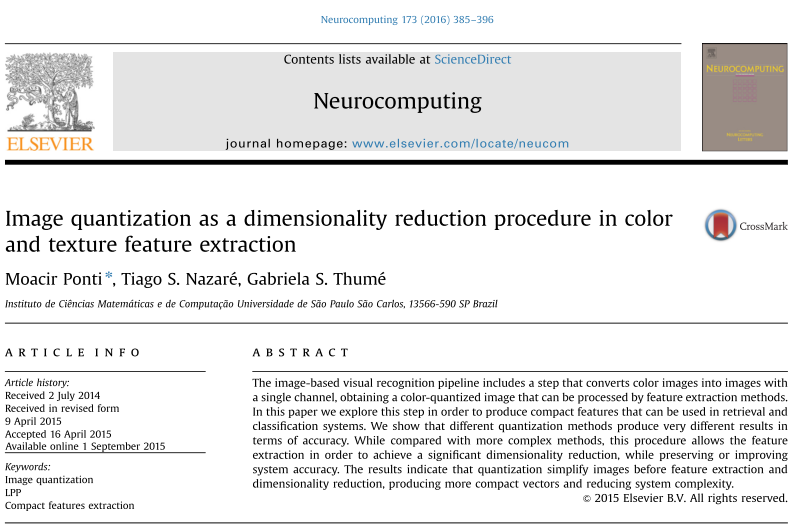
\includegraphics[width=\linewidth]{figuras/artigo.png}
 \end{center}
 \caption{Artigo publicado na \textit{Neurocomputing}, referente a quantização de imagens. \textit{Fonte~\url{http://www.sciencedirect.com/science/article/pii/S0925231215012771}}.}
 \label{fig:artigo}
\end{figure}

\section{Trabalhos Futuros}

% TODO: Sugerir em trabalhos futuros, no cap de Conclusão, um SMOTE visual não-aleatório: tomando-se imagens próximas, assim como é feito no SMOTE, dada uma medida de distância qualquer (k-means, euclidiana?)

Ao usar imagens com reduzido número de cores (quantizadas), os métodos de extração de características baseados em orientação (HoG, SIFT), \textit{bag of visual words} e \textit{Fisher vectors}, seriam provavelmente mais esparços.
\meutodo{trabalhos futuros da quantização}

Como extensão dos experimentos reportados pode ser feita a análise dos espaços encontrados para os diferentes métodos de geração artificial de imagens. Além disso, o impacto de tais métodos em diferentes extratores de características pode sugerir quais são as características latentes percebidas com cada extrator.

Atualmente, o estado da arte de extração e classificação de imagens corresponde ao uso de redes neurais de convolução, conhecidas por CNN \cite{Schmidhuber2014}. Essas redes são compostas por camadas de neurônios que têm por objetivo aprender quais são as melhores características que diferenciam as classes de imagens. O aprendizado, nesse caso, corresponde ao ajuste dos parâmetros para reduzir a diferença entre a saída esperada -- classe verdadeira -- e a produzida. Dessa forma, tais redes aprendem quais são as características latentes nas imagens de entrada. Uma possível continuação a esta pesquisa é analisar as características aprendidas por uma CNN. Essa rede permite encontrar as características mais relevantes da base de imagens, que os extratores de características canônicos não capturam. Isso porque ela possui uma hierarquia de camadas, desde a imagem original até uma etapa de classificação, com o objetivo de aprender qual o melhor processamento para as imagens de modo a melhor discriminar as classes. Podem também indicar possíveis operações para auxiliar na geração de imagens artificiais.

Além de analisar o processamento realizado por uma rede de convolução para a classificação das imagens, uma RBM (máquinas de Boltzmann restritas) também pode ser treinada para análise da sua memória associativa (matriz de características aprendida). Uma rede neural RBM treina um modelo a partir dos vetores de entrada \cite{Fischer2014}. As imagens artificialmente geradas foram adicionadas no conjunto de treino sem verificação da sua relevância, o que pode ter prejudicado a classificação. A representação das imagens de entrada, aprendida pela etapa de treinamento da RBM, pode ser utilizada para definir quais imagens são relevantes para o aprendizado ou não. Além disso, pode servir como escolha para qual imagem original utilizar, ao invés do método aleatório utilizado nos resultados preliminares.

\meutodo{adicionar figuras de visualização do espaço correspondente a adição de cada tipo diferente de imagem gerada?}
